\documentclass[10pt]{article}
\usepackage[margin=0.75in]{geometry}
\usepackage{graphicx}
\usepackage{booktabs}
\usepackage{amsmath}
\usepackage{caption}
\usepackage{hyperref}
\setlength{\parskip}{0.3em}
\setlength{\parindent}{0pt}
\renewcommand{\arraystretch}{1.15}
\setlength{\tabcolsep}{6pt}

\title{\vspace{-1.5em}COL774 Assignment 1 --- Report}
\author{}
\date{}

\begin{document}
\maketitle
\vspace{-3em}

\section*{1. Created Features}

\textbf{Part (c) --- Heart rate from BVP/accelerometer/EDA.}
\begin{center}
\footnotesize
\begin{tabular}{lp{2.5cm}lp{6.5cm}}
\toprule
Feature & Full name & Modality & Explanation \\
\midrule
\texttt{acf\_lag\{20..85\}} & Pulse Self-Similarity Curve (66) & BVP (wrist pulse) & How closely the pulse wave matches a delayed copy of itself, checked at every delay a plausible heart rate could produce. This directly reveals the true beat rate. \\
\texttt{acf\_peak\_*} & Best-Match Summary (3) & BVP (wrist pulse) & The strongest match point on that curve, and the heart rate it points to. \\
\texttt{bvp\_mean...zc} & Pulse Wave Shape (8) & BVP (wrist pulse) & How strong, spread out, and jagged the raw pulse wave looks. \\
\texttt{acc\_*} & Wrist Motion (10) & Accelerometer & How much, and in what pattern, the wrist is moving -- movement can distort the pulse reading. \\
\texttt{eda\_mean...slope} & Sweat Response (4) & EDA (skin) & Overall sweat-response level, how much it varies, and its trend. \\
\bottomrule
\end{tabular}
\end{center}

\textbf{Part (d) --- CGM glucose from Empatica E4 + Zephyr BioHarness.} \textbf{Final model:}
LassoCV, 5-fold CV over a 30-point log-spaced $\alpha$ grid, features standardized before fitting.
\begin{center}
\footnotesize
\begin{tabular}{lp{3.0cm}lp{6.4cm}}
\toprule
Feature & Full name & Modality & Explanation \\
\midrule
\texttt{bvp\_*} & Pulse Wave Shape \& Timing (17) & BVP (wrist pulse) & What the pulse wave looks like and how steady the timing between heartbeats is. \\
\texttt{e4\_hr\_*} & Device Heart Rate (7) & Heart rate (wrist sensor) & The wristband's own heart-rate reading, and whether it drifts during the window. \\
\texttt{eda\_*} & Sweat Response (19) & EDA (skin) & How much someone is sweating, and what sudden ``stress spike'' events look like. \\
\texttt{temp\_*} & Skin Temperature (8) & Temperature & How skin temperature shifts within the window (each person's own baseline removed). \\
\texttt{e4\_acc\_sq\_*, bvp\_motion\_quality} & Wrist Motion \& Signal Quality (6) & Accelerometer (wrist) & How much the wrist is moving, and whether that motion is corrupting the pulse reading. \\
\texttt{ecg\_mean...sampen} & Heartbeat Waveform \& Rhythm (18) & ECG (chest strap) & The heartbeat's electrical shape and how its timing varies -- linked to the body's stress/calm balance. \\
\texttt{ecg\_qt\_*, qtc\_*, t\_*} & Heart's Electrical Recovery Time (6) & ECG (chest strap) & How long the heart takes to ``reset'' after each beat -- known to lengthen during low blood sugar. \\
\texttt{ptt\_mean, ptt\_std} & Pulse Travel Time (2) & ECG + BVP together & How long the pulse takes to travel from the heart to the wrist. \\
\texttt{zephyr\_acc\_sq\_*, ecg\_motion\_quality} & Chest Motion \& Signal Quality (6) & Accelerometer (chest) & How much the chest strap is moving, and whether that's corrupting the ECG reading. \\
\texttt{breathing\_*} & Breathing Pattern (13) & Breathing (chest strap) & How breathing depth, rate, and trend change within the window. \\
\bottomrule
\end{tabular}
\end{center}

\section*{2. Normalized Acceleration}

Figure~\ref{fig:parta} shows a representative Part (a) window (BVP, $\tilde{a}_{sq}(t)$, EDA,
target HR); Figure~\ref{fig:partd} shows a representative Part (d) window (BVP,
$\tilde{a}_{sq}(t)$, EDA, ECG, on-device heart rate, target CGM glucose). In the Part (d) window,
two motion episodes (visible as spikes in $\tilde{a}_{sq}(t)$ around $t{=}40$--$110$s) coincide
with BVP/EDA artifact and a heart-rate rise -- exactly the motion-corruption effect the
signal-quality ratio features are designed to flag.

\begin{figure}[h]
  \centering
  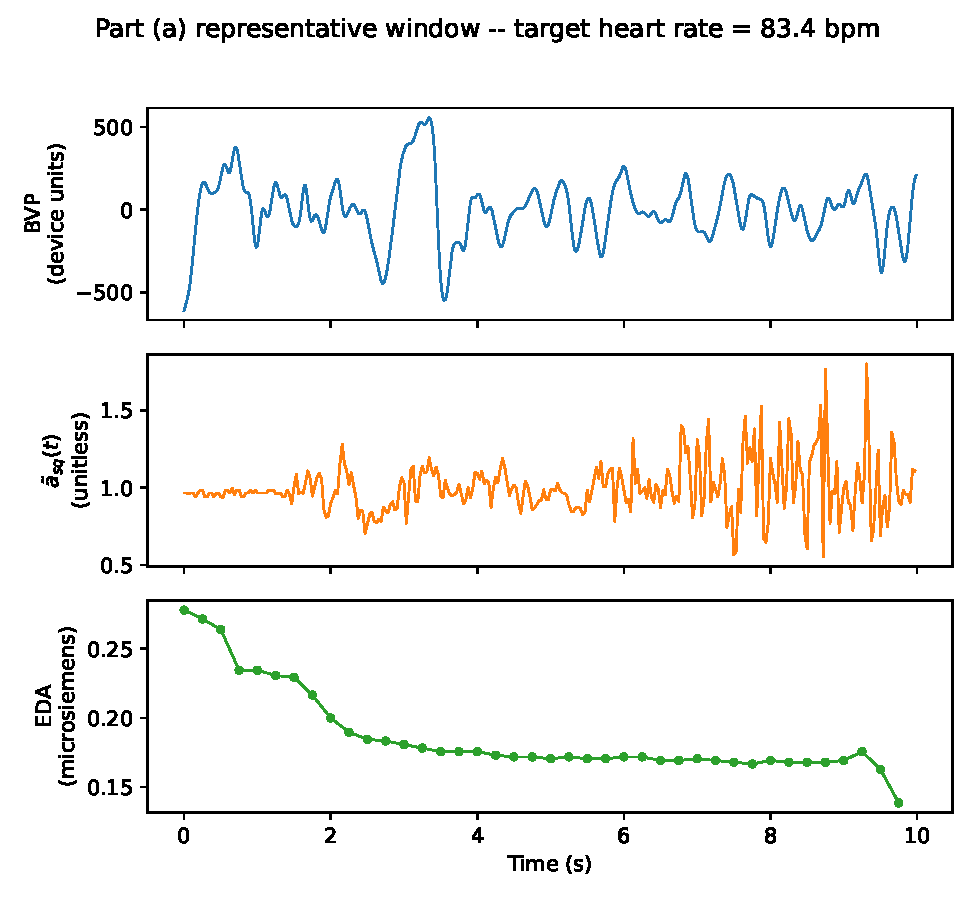
\includegraphics[width=0.46\linewidth]{report_assets/part_a_window.pdf}
  \caption{Representative Part (a) window.}
  \label{fig:parta}
\end{figure}

\begin{figure}[h]
  \centering
  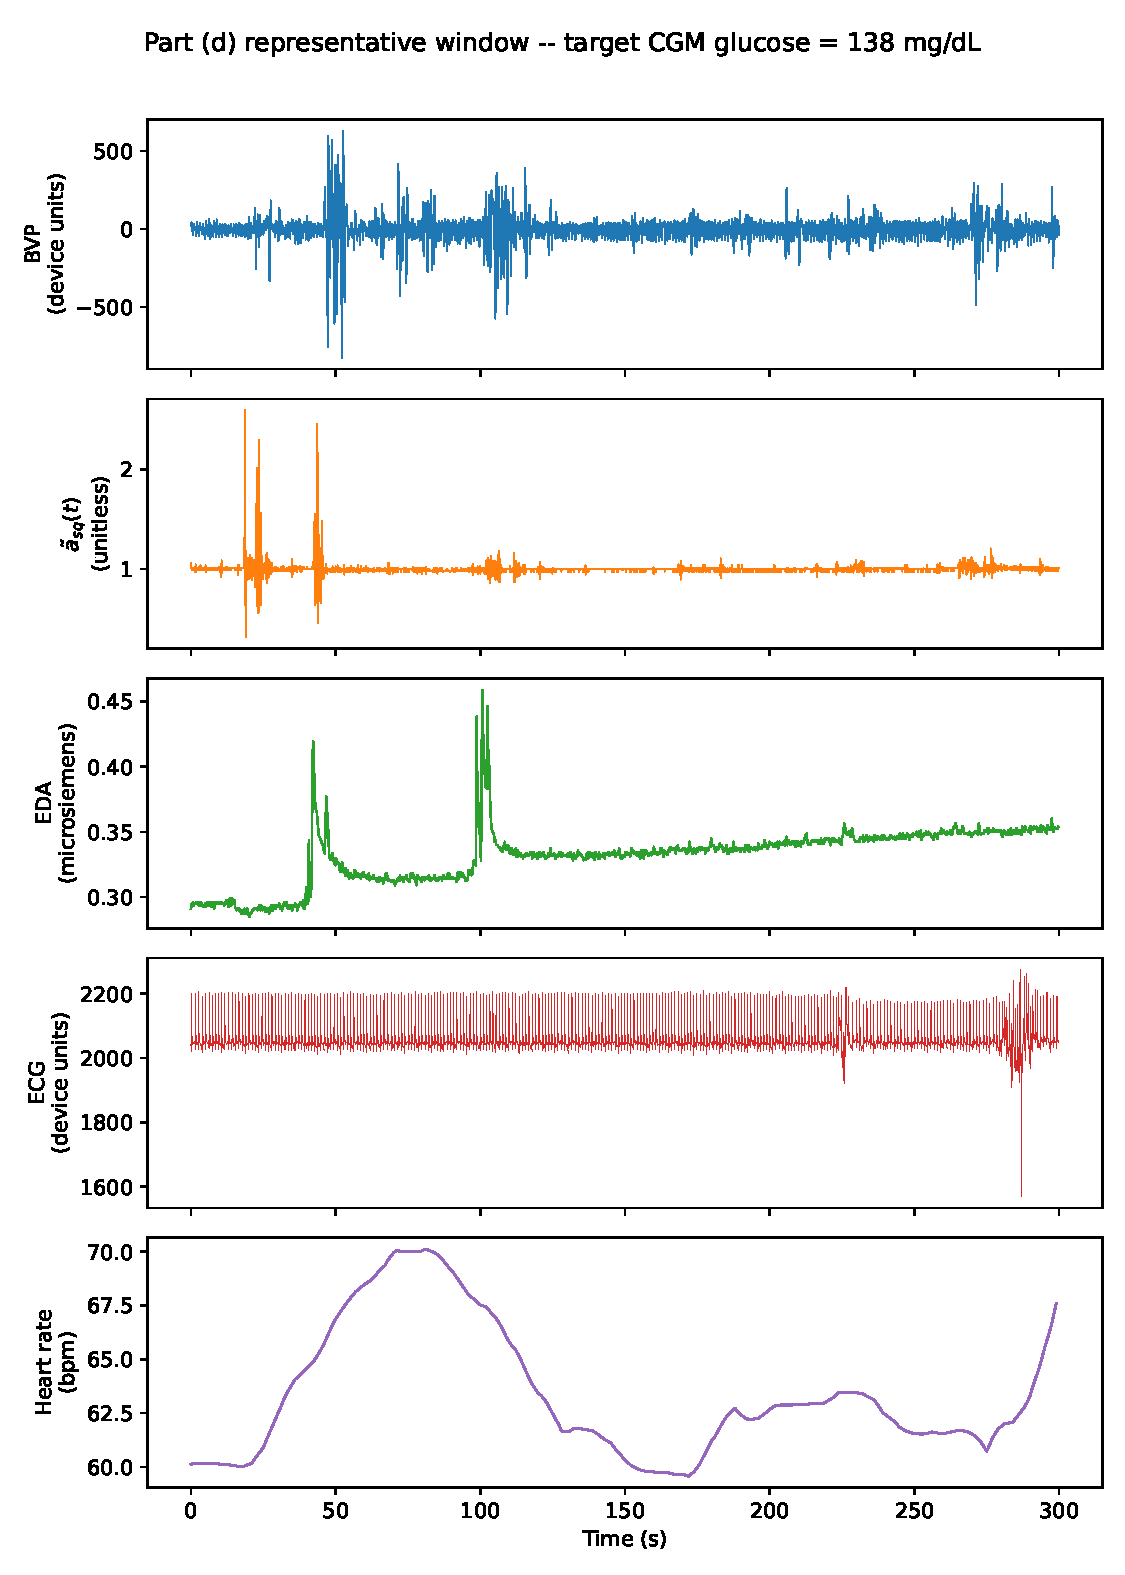
\includegraphics[width=0.5\linewidth]{report_assets/part_d_window.pdf}
  \caption{Representative Part (d) window.}
  \label{fig:partd}
\end{figure}

\section*{3. Top Five Features}

Importance is $|\text{standardized regression coefficient}|$ (features standardized before
comparison), per PDF instructions.

\textbf{Part (c)} (Ridge, $\alpha{=}0.01$):
\begin{center}
\small
\begin{tabular}{llrp{6.1cm}}
\toprule
Feature & Modality & $|$std.\ coef.$|$ & Why relevant \\
\midrule
\texttt{acf\_lag28} & BVP (autocorrelation) & 101.13 & Match strength at the delay corresponding to $\approx$137~bpm -- close to this window's actual heart rate. \\
\texttt{acf\_lag50} & BVP (autocorrelation) & 98.34 & Match strength at the $\approx$77~bpm delay. \\
\texttt{acf\_lag26} & BVP (autocorrelation) & 89.64 & Match strength at the $\approx$148~bpm delay. \\
\texttt{acf\_lag48} & BVP (autocorrelation) & 78.92 & Match strength at the $\approx$80~bpm delay. \\
\texttt{acf\_lag30} & BVP (autocorrelation) & 78.79 & Match strength at the $\approx$128~bpm delay. \\
\bottomrule
\end{tabular}
\end{center}
Several adjacent-lag ACF values receiving large, opposite-sign coefficients lets the linear model
interpolate the true period at sub-sample resolution, rather than relying on one discrete peak lag.

\textbf{Part (d)} (LassoCV; protocol d3, cross-subject -- the hardest, most heavily-weighted
split):
\begin{center}
\small
\begin{tabular}{llrp{5.7cm}}
\toprule
Feature & Modality & $|$std.\ coef.$|$ & Why relevant \\
\midrule
\texttt{ecg\_qt\_mean} & ECG (Zephyr) & 7.38 & How long the heart takes to ``reset'' after each beat -- this stretches out during low blood sugar in Type~1 diabetes. \\
\texttt{ecg\_min} & ECG (Zephyr) & 1.57 & The lowest point of the heartbeat's electrical waveform (each person's own baseline removed). \\
\texttt{breathing\_std} & Breathing (Zephyr) & 1.18 & How much breathing depth varies within the window (baseline removed). \\
\texttt{ecg\_lf\_hf\_ratio} & ECG HRV (Zephyr) & 0.74 & Balance between the body's ``alert'' and ``calm'' nervous-system activity; expected to shift during a glucose swing. \\
\texttt{ecg\_sd1\_sd2\_ratio}$^{*}$ & ECG HRV (Zephyr) & 0.37 & A geometric comparison of short-term vs.\ longer-term heartbeat-timing variability. \\
\bottomrule
\end{tabular}
\end{center}
{\footnotesize $^{*}$Lasso keeps only 4 features nonzero in the d3 fit (the four above it); the 5th
is the strongest signal from the d2 fit -- overall, importance concentrates almost entirely in
ECG timing/HRV and breathing.}

\section*{4. Median Baseline Comparison}

\begin{center}
\small
\begin{tabular}{lrrrr}
\toprule
& \multicolumn{2}{c}{Model} & \multicolumn{2}{c}{Median baseline} \\
Part / Protocol & NMAE & NMSE & NMAE & NMSE \\
\midrule
Part (c) (local val., $n{=}31{,}797$)      & 0.6434 & 0.5002 & 0.9918 & 1.0141 \\
Part (d), d1 (random within-subject)       & 0.9277 & 0.9056 & 0.9709 & 1.0624 \\
Part (d), d2 (temporal within-subject)     & 0.9328 & 0.9592 & 0.9951 & 1.1429 \\
Part (d), d3 (cross-subject)               & 1.0038 & 1.0935 & 1.0958 & 1.3660 \\
\bottomrule
\end{tabular}
\end{center}

\end{document}
